\section{Materials and Methods}

To develop the benchmark for electrodes in BioZ and BCC application, first of all we need to identify what are the parameters we are seeking. In other words, if we have ideal signal, what are parameters of that signal, and what changes of those parameters would lead to reduction of quality of the signal.

Starting our thought experiment with pure sine wave, with zero noise, and amplitude high enought, so the smallest changes in that sine-wave would be captured by our ideal ADC.

Now lets observe real life measurements (See figures \ref{fig:agagcl_breathing}, \ref{fig:edigold_breathing}, \ref{fig:movsense_breathing}) and try to identify what are those elements that separates real world form ideal. 

\begin{figure}
    \centering
    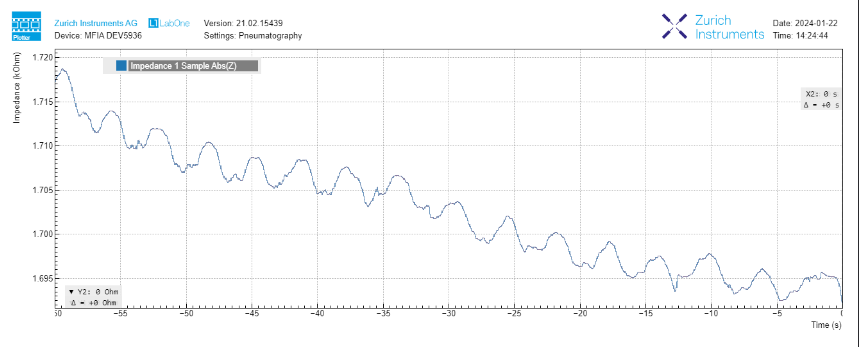
\includegraphics[width=1.2\linewidth]{figures/PlaceHolders/AgAgCl_Placeholder.png}
    \caption{AgAgCl electrodes capturing breathing}
    \label{fig:agagcl_breathing}
\end{figure}

\begin{figure}
    \centering
    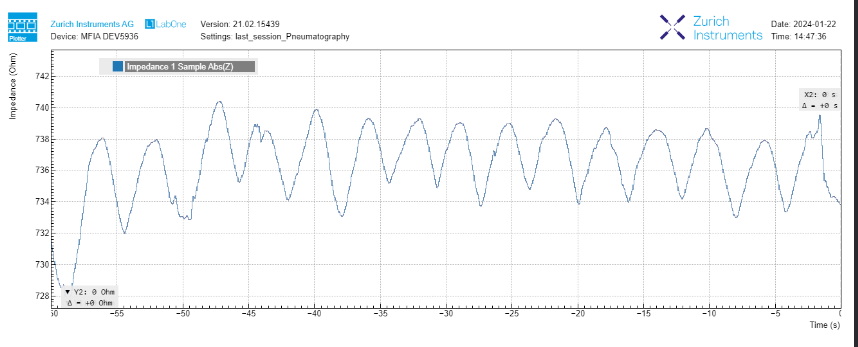
\includegraphics[width=1.2\linewidth]{figures/PlaceHolders/EDI_Gold_Placeholder.png}
    \caption{Custom, gold plated electrodes capturing breathing}
    \label{fig:edigold_breathing}
\end{figure}

\begin{figure}
    \centering
    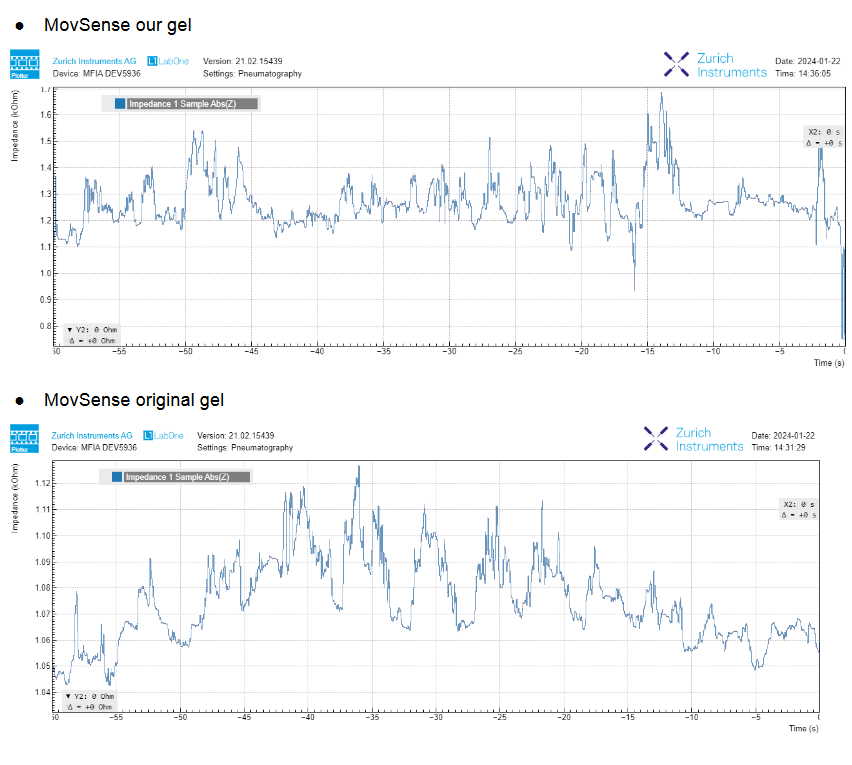
\includegraphics[width=1.2\linewidth]{figures/PlaceHolders/MovSense_Placeholder.png}
    \caption{Unknown electrodes from our shelf, we completely have no idea who is the manufacturer of those electrodes}
    \label{fig:movsense_breathing}
\end{figure}

Looking at \ref{fig:agagcl_breathing}, we see that "amplitude of inhale-exhale" is about 5 ohms, the measurement drifts from 1.72KOhm to 1.695KOhms over one minute. There is insignificant noise, about 0.1 Ohm and breathing pattern is clearly visible.



\input{sections/011_participants.tex}
\input{sections/012_equipment.tex}
% ... more subsections as needed
